%%%%%%%%%%%%%%%%%%%%%%%%%%%%%%%%%%%%%%%%%
% Beamer Presentation
% LaTeX Template
% Version 1.0 (10/11/12)
%
% This template has been downloaded from:
% http://www.LaTeXTemplates.com
%
% License:
% CC BY-NC-SA 3.0 (http://creativecommons.org/licenses/by-nc-sa/3.0/)
%
%%%%%%%%%%%%%%%%%%%%%%%%%%%%%%%%%%%%%%%%%

%----------------------------------------------------------------------------------------
%	PACKAGES AND THEMES
%----------------------------------------------------------------------------------------

\documentclass{beamer}

\mode<presentation> {

% The Beamer class comes with a number of default slide themes
% which change the colors and layouts of slides. Below this is a list
% of all the themes, uncomment each in turn to see what they look like.

%\usetheme{default}
%\usetheme{AnnArbor}
%\usetheme{Antibes}
%\usetheme{Bergen}
%\usetheme{Berkeley}
%\usetheme{Berlin}
%\usetheme{Boadilla}
%\usetheme{CambridgeUS}
%\usetheme{Copenhagen}
%\usetheme{Darmstadt}
%\usetheme{Dresden}
%\usetheme{Frankfurt}
%\usetheme{Goettingen}
%\usetheme{Hannover}
%\usetheme{Ilmenau}
%\usetheme{JuanLesPins}
%\usetheme{Luebeck}
\usetheme{Madrid}

\usepackage{listings} % Required for insertion of code
%\usetheme{Malmoe}
%\usetheme{Marburg}
%\usetheme{Montpellier}
%\usetheme{PaloAlto}
%\usetheme{Pittsburgh}
%\usetheme{Rochester}
%\usetheme{Singapore}
%\usetheme{Szeged}
%\usetheme{Warsaw}

% As well as themes, the Beamer class has a number of color themes
% for any slide theme. Uncomment each of these in turn to see how it
% changes the colors of your current slide theme.

%\usecolortheme{albatross}
%\usecolortheme{beaver}
%\usecolortheme{beetle}
%\usecolortheme{crane}
%\usecolortheme{dolphin}
%\usecolortheme{dove}
%\usecolortheme{fly}
%\usecolortheme{lily}
%\usecolortheme{orchid}
%\usecolortheme{rose}
%\usecolortheme{seagull}
%\usecolortheme{seahorse}
%\usecolortheme{whale}
%\usecolortheme{wolverine}

%\setbeamertemplate{footline} % To remove the footer line in all slides uncomment this line
%\setbeamertemplate{footline}[page number] % To replace the footer line in all slides with a simple slide count uncomment this line

%\setbeamertemplate{navigation symbols}{} % To remove the navigation symbols from the bottom of all slides uncomment this line
}

\usepackage{graphicx} % Allows including images
\usepackage{booktabs} % Allows the use of \toprule, \midrule and \bottomrule in tables

%----------------------------------------------------------------------------------------
%	TITLE PAGE
%----------------------------------------------------------------------------------------

\title[Introduzione]{Threads} % The short title appears at the bottom of every slide, the full title is only on the title page

\author{Claudio Menghi,  Srdan Krstic} % Your name
\institute[Deepse group] % Your institution as it will appear on the bottom of every slide, may be shorthand to save space
{
Politecnico di Milano \\ % Your institution for the title page
\medskip
\textit{menghi@elet.polimi.it,  srdan.krstic@polimi.it} % Your email address
}
\date{\today} % Date, can be changed to a custom date

\begin{document}

\begin{frame}
\titlepage % Print the title page as the first slide
\end{frame}

\begin{frame}
\frametitle{Overview} % Table of contents slide, comment this block out to remove it
\tableofcontents % Throughout your presentation, if you choose to use \section{} and \subsection{} commands, these will automatically be printed on this slide as an overview of your presentation
\end{frame}

%----------------------------------------------------------------------------------------
%	PRESENTATION SLIDES
%----------------------------------------------------------------------------------------



\section{Threads}
\begin{frame}
\frametitle{Threads}
\begin{itemize}
\item I computer odierni possono eseguire pi\`u di un processo alla volta. 
\item Anche un singolo processo pu\`o eseguire pi\`u operazioni in contemporanea. 
\item La piattaforma Java fornisce un supporto per lo sviluppo di sistemi concorrenti. Tale supporto \`e contenuto nel package \emph{java.util.concurrent}.
\end{itemize}
\end{frame}

\begin{frame}
\frametitle{Threads}
In un sistema concorrente ci sono due diversi tipi ti elementi che possono essere eseguiti: \emph{processi} e \emph{threads}. 
\begin{itemize}
\item \emph{processi} sono ambienti di esecuzione self-contained, a un set di risorse private a run-time e in particolare ha il suo \emph{spazio in memoria}. Per comunicare pi\`u processi hanno bisogno di sockets.
\item \emph{threads} sono ``processi a basso costo" richiedono meno risorse, esistono all'interno di \emph{un} processo e condividono le risorse, i file parti etc. Questo rende molto efficiente la comunicazione tra i threads ma sotto un certo aspetto pi\`u problematica. Ogni applicazione \`e associata ad almeno un thread principale che pu\`o chiamare pi\`u thread secondari.
\end{itemize}
\end{frame}

\begin{frame}
\frametitle{Thread in Java}
Ci sono due strategie per creare un thread:
\begin{itemize}
\item \emph{creare un oggetto runnabile}: basta implementare l'interfaccia \emph{Runnable}: ci forza a implementare il metodo \emph{run} che contiene il codice eseguito dal thread.  Per creare il thread \`e sufficiente istanziare un oggetto di classe \texttt{Thread} a cui viene passato il riferimento all'oggetto runnabile. 
\item \emph{estendere la classe Thread}: la classe thread ha un implementazione di default del metodo \texttt{run} che non fa nulla. \`E necessario overridare il metodo \texttt{run} della classe \texttt{Thread}. Attenzione, se la vostra classe estende \texttt{Thread} non pu\`o estendere un altra classe, per questo la prima scelta \`e pi\`u generale.
\end{itemize}
\end{frame}

\begin{frame}
\frametitle{Metodi di thread}
\begin{itemize}
\item \emph{start}: avvia il thread (eseguendo il metodo run)
\item \emph{join}: un thread si mette in attesa della terminazione del thread su cui \`e invocato
\item \emph{isAlive}: controlla se il thread \`e vivo (in esecuzione, in attesa o bloccato)
\item \emph{sleep(int ms)}: sospende l’esecuzione del thread sospende l’esecuzione del thread corrente
\item \emph{yield}: cede la precedenza
\end{itemize}
\end{frame}

\begin{frame}
\frametitle{Altri metodi utili}
\begin{itemize}
\item \emph{wait}: sospende il thread corrente. Il thread non viene risvegliato finch\`e non gli arriva una notifica.
\end{itemize}
Due metodi possono essere utilizzati per svegliare i thread
\begin{itemize}
\item \emph{notifyAll}: manda una notifica a \emph{tutti} i thread che sono in sleep in attesa di quel lock. I thread corrispondenti si svegliano.
\item \emph{notify}: sveglia un singolo thread non deterministicamente
\end{itemize}
\end{frame}

\begin{frame}
\frametitle{Stati di un thread}
\begin{itemize}
\item \emph{born} \`e lo stato che viene raggiunto dopo che  viene eseguita l'istruzione 
\texttt{Thread t=new Thread(Runnable target, String name);}
\item \emph{ready} viene raggiunto quando viene invocato il metodo start sull'oggetto. In questo stato il thread non st\`a eseguendo nulla, \`e solo pronto ad eseguire il codice.
\item \emph{running} viene raggiunto quando effettivamente il codice all'interno di run viene eseguito. 
\item \emph{sleep} quando viene invocato il metodo sleep sul thread. Non c'\`e garanzia che il thread v\`a in sleep esattamente nel momento che invoco il metodo. 
\item \emph{waiting} un thread viene messo in questo stato quando viene invocato il metodo \texttt{wait}
\item \emph{blocked} il thread \`e bloccato quando attende un particolare lock monitorato o di accedere a un metodo synchronized. Viene messo in questo stato anche dopo che viene risvegliato dal wait
\item \emph{dead} quando il thread \`e terminato. Non \`e pi\`u possibile invocare il metodo start su un thread terminato.
\end{itemize}
\end{frame}

\begin{frame}
\frametitle{Stati di un thread}
\begin{figure}[h!]
  \centering
    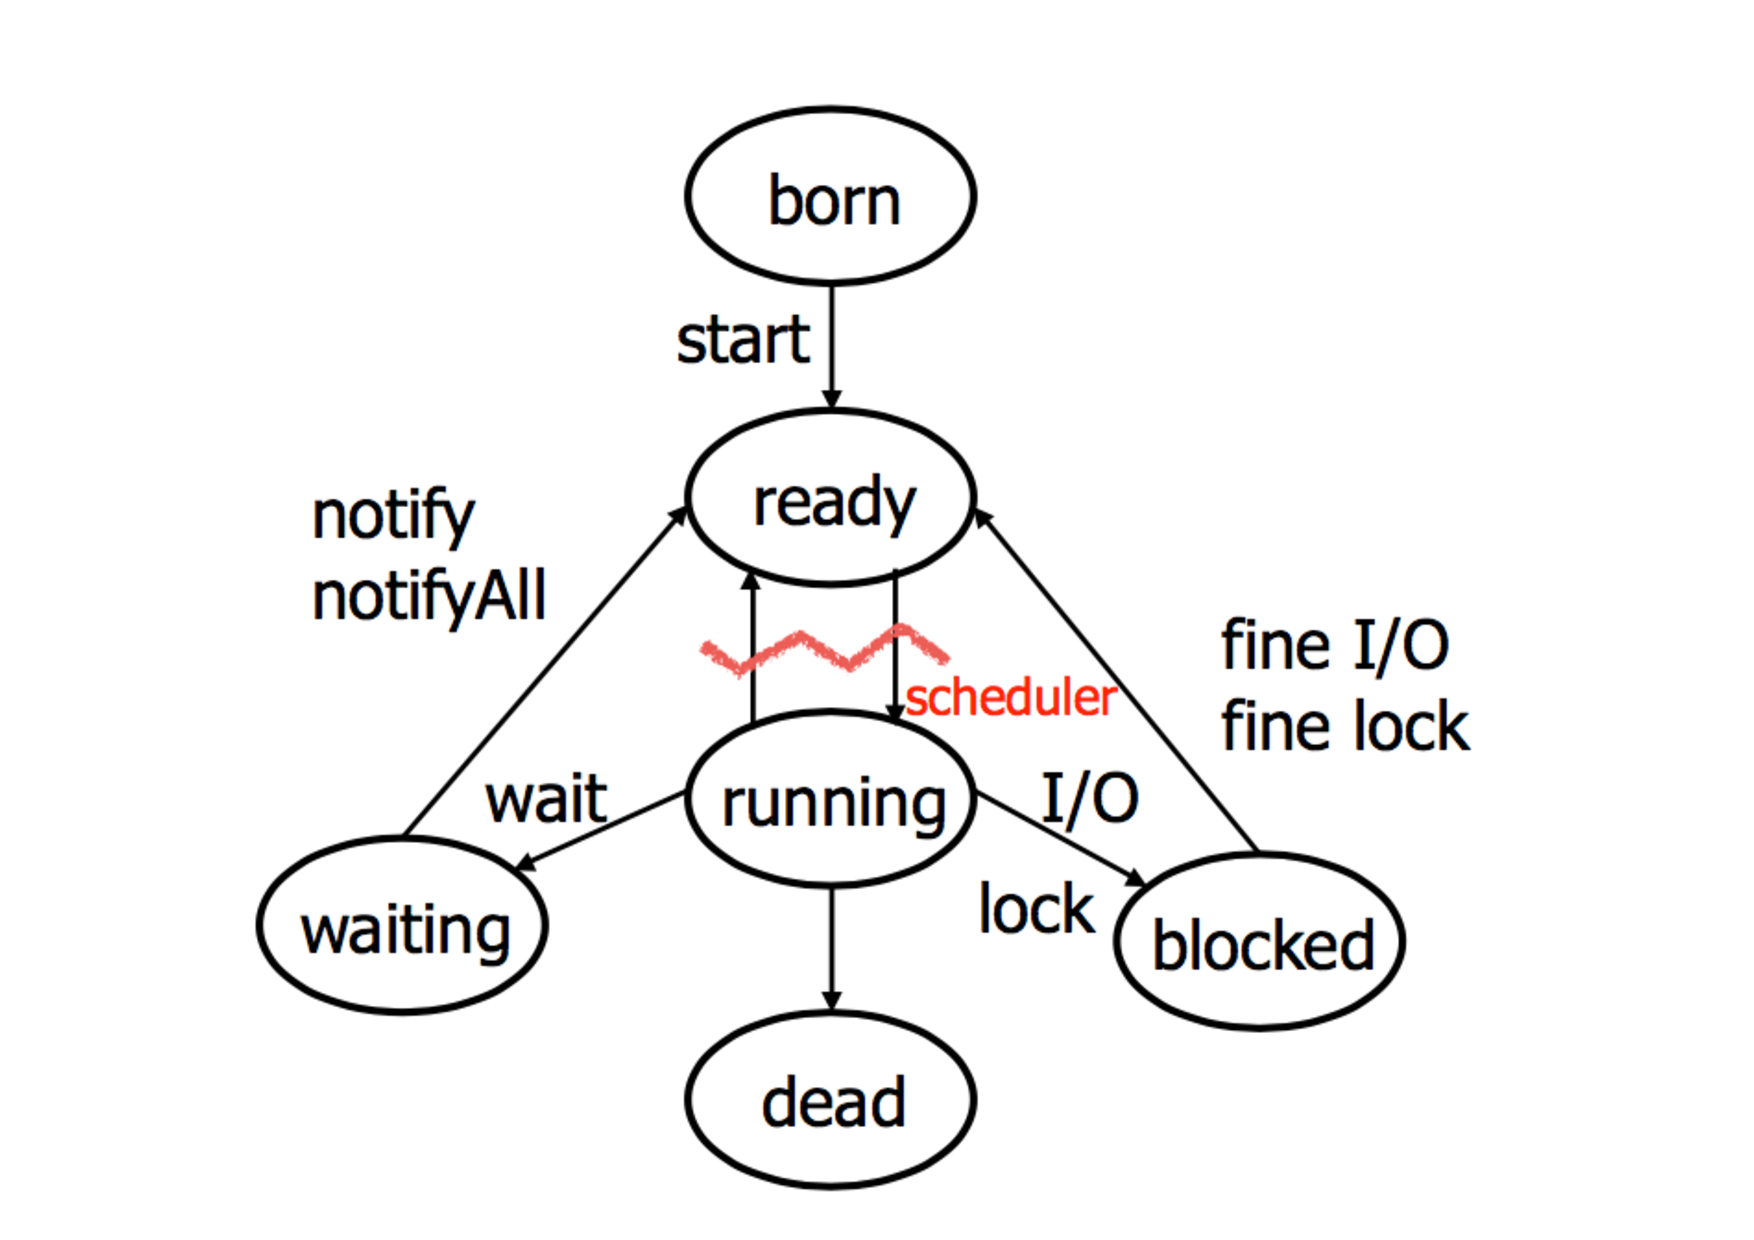
\includegraphics[width=0.8\textwidth]{stati.pdf}
\end{figure}

\end{frame}

\begin{frame}
\frametitle{Problemi nell'utilizzo dei threads}
\begin{itemize}
\item \emph{interferenze}: sono dovuti al fatto che diversi thread lavorano in parallelo sugli stessi dati
\end{itemize}
\end{frame}





\begin{frame}
\frametitle{Risolvere le interferenze}
Per risolvere le interferenze abbiamo due strategie:
\begin{itemize}
\item Metodi synchronized
\item Blocchi/statements synchronized
\end{itemize}
\end{frame}

\begin{frame}
\frametitle{Risolvere le interferenze}
Metodi synchronized:
\begin{itemize}
\item l'esecuzione di metodi syncronized \textbf{di uno stesso oggetto} non pu\`o sovrapporsi
\item un metodo pu\`o essere eseguito solo dopo che il precedente termina
\item utilizzano il lock intrinseco dell'oggetto
\end{itemize}
\end{frame}

\begin{frame}
\frametitle{Risolvere le interferenze}
 Blocchi/statements synchronized
\begin{itemize}
\item hanno una granularit\`a pi\`u fine: a volte solo una porzione del metodo deve essere sincronizzata
\item anzich\`e rendere atomico tutto il metodo \`e possibile rendere atomico un sottoblocco
\end{itemize}
\end{frame}



\begin{frame}
\frametitle{Lock Objects}
Sono pi\`u di alto livello rispetto ai lock normali. Per esempio permeddono di specificare condizioni sui lock implementando l'interfaccia \texttt{Condition}

Inoltre, con i lock object \`e possibile utilizzare 
\begin{itemize}
\item il metodo \texttt{tryLock} che prova a prendere il lock e se non lo ottiene ritorna invece di mandare il thread in wait
\item il metodo \texttt{lockInterruptibly} consente il ritiro di un thread se un altro thread manda un interrupt prima che il lock sia acquisito.
\end{itemize}
\end{frame}


\begin{frame}
\frametitle{Esecutori}
Ci sono 3 diverse interfacce che consentono di gestire i thread mediante esecutori
\begin{itemize}
\item Executor: interfaccia che permette di lanciare nuovi task. . Un elemento di tipo executor offre il metodo \texttt{execute(Runnable command)} che consente di eseguire un elemento runnable. 
\item ExecutorService: aggiunge nuove features agli executors, per esempio fornisce metodi quali \texttt{submit(Runnable task)} che submitta un task per l'esecuzione o \texttt{shutdown} il quale inizia lo spegnimento (nuovi task non sono accettati quelli gi\`a in coda sono finiti).
\item ScheduledExecutorServece: interfaccia permette di specificare informazioni addizioali come una politica di scheduling dei vari threads.
\end{itemize}
\end{frame}

\begin{frame}
\frametitle{Thread Pools}
Sono utilizzati all'interno di maggior parte degli executors. Sono creati per \emph{minimizzare} l'overhead richiesto alla creazione dei threads, visto che la gestione dei threads richiede un significativo quantitativo di memoria. In genere forniscono un insieme \emph{pool} di threads gi\`a preistanziato o riusano i thread terminati
\end{frame}

\begin{frame}
\frametitle{Usare executors}
Per creare un Executor \`e possibile utilizzare i metodi statici contenuti all'interno della classe \texttt{Executors}. Per esempio, \texttt{Executors.newFixedThreadPool(int nThreads)} restituisce un thread pool con un numero di thread predefiniti. In particolare, potrebbero essere utili:
\begin{itemize}
\item SingleThreadExecutor: esegue un solo task alla volta
\item FixedThreadPool: esegue un numero fissato di task in parallelo
\item CachedThreadPool: esegue un numero illimitato di task in parallelo
\item ScheduledThreadPool: permette di programmare l’esecuzione dei task
\end{itemize}
\end{frame}


\begin{frame}
\frametitle{Collezioni sincrone}
La maggior parte delle collezioni e mappe che abbiamo visto finora non sono thread-safe. 
\begin{itemize}
\item esitono delle versioni delle collezioni thread safe 
\item ovviamente hanno prestazioni peggiori. 
\item Per ottenere una lista sincronizzata \`e possibile per esempio utilizzare il metodo statico \texttt{Collections.synchronizedList(List<T> list)} di \texttt{Collections}. 
\item Interessanti sono anche le classi \texttt{CopyOnWriteArrayList} e simili, utili quando non si vuole rendere sincrona l'operazione di iterazione ma solo la modifica della lista. Queste classi sono contenute in \texttt{java.util.concurrent}.
\end{itemize}
\end{frame}

\begin{frame}
\frametitle{Variabili atomiche}
Il package java.util.atomic definisce classi che supportano operazioni atomiche su singole variabili per esempio \texttt{AtomicBoolean}.
\begin{itemize}
\item Esse posseggono tutte metodi get e set che si comportano come lettura e scrittura delle corrispondenti variabili non atomiche
\item E' disponibile anche un'operazione \texttt{compareAndSet}
\end{itemize} 
\end{frame}

\begin{frame}
\frametitle{Problemi nell'utilizzo della sincronizzazione}
\begin{itemize}
\item \emph{liveness} un applicazione viene eseguita entro accettabili vincoli di tempo, sue sottopropriet\`a sono:
\begin{itemize}
\item \emph{deadlock}: due thread sono bloccati uno in attesa dell'altro
\item \emph{starvation}:un thread ha difficolt\`a a prendere la risorsa, gli altri thread spendono molto tempo o hanno uno scheduler che li aiuta
\item \emph{livelock}: genera una sequenza ciclica di operazioni inutili 
\end{itemize}
\end{itemize}
\end{frame}

\section{Esercizi}
\begin{frame}
\frametitle{Esercizio 1}
Modellizzare una sala da ballo. All'interno della sala da ballo ci sono delle Dame, ognuna dell quali pu\`o essere in due stati: \texttt{IN\_COPPIA} o \texttt{SENZA\_UOMO}. Un cavaliere sceglie una dama dalla sala e le chiede di ballare. Se la dama ha gi\`a un cavaliere, ritorna \texttt{false}, altrimenti la dama \`e libera di ritornare \texttt{true} o \texttt{false} in relazione al gradimento per il cavaliere. Dopo aver eseguito un ballo (pi\`u o meno lungo) il cavaliere rilascia la dama.
\end{frame}
\begin{frame}
\frametitle{Esercizio 2}
Quando una dama \`e occupata in un altro ballo il cavaliere si mette in attesa che la dama desginata si liberi. Nota che non \`e detto che una volta libera la dama si conceda al cavaliere (potrebbe esserci un altro cavaliere in attesa pi\`u lesto o semplicemente il cavaliere non \`e di gradimento della dama).
\end{frame}

\begin{frame}
\frametitle{Esercizio 3}
Quando una dama \`e occupata in un altro ballo il cavaliere si mette in attesa che la dama desginata si liberi. Nota che non \`e detto che una volta libera la dama si conceda al cavaliere (potrebbe esserci un altro cavaliere in attesa pi\`u lesto o semplicemente il cavaliere non \`e di gradimento della dama).
\end{frame}

\begin{frame}
\frametitle{Esercizio 4}
Prima che la donna si conceda a un ballo \`e necessario spendere del tempo nel corteggiamento (il metodo risponde \`e un attivit\`a lunga). Un cavaliere, quando vede che la dama desiderata \`e corteggiata da un altro cavaliere si demoralizza e non vuole attendere oltre. 
\end{frame}

\begin{frame}
\frametitle{Esercizio 5}
La sala da ballo pu\`o contenere al pi\`u 3 cavalieri per volta 
\end{frame}


%----------------------------------------------------------------------------------------

\end{document} 